\documentclass[14pt]{beamer}
\usepackage{graphicx}
\usepackage{hyperref}
\usepackage{xcolor}
\graphicspath{ {./images/} }

\title{MaskifAI}
\subtitle{A mask detection web app}
\author[TEAM 6]{Sachita Malhotra, Shruthi Rao, Srishti Negi}
\date{June - August 2020}


\usetheme{AnnArbor}

\newcounter{saveenumerate}
\newcommand{\saveenumerate}{\setcounter{saveenumerate}{\value{enumi}}}
\newcommand{\restartenumerate}{\setcounter{enumi}{\value{saveenumerate}}}

\begin{document}

\begin{frame}
    \titlepage
\end{frame}

\begin{frame}
    \frametitle{Where would you feel safer?}
    \centering
    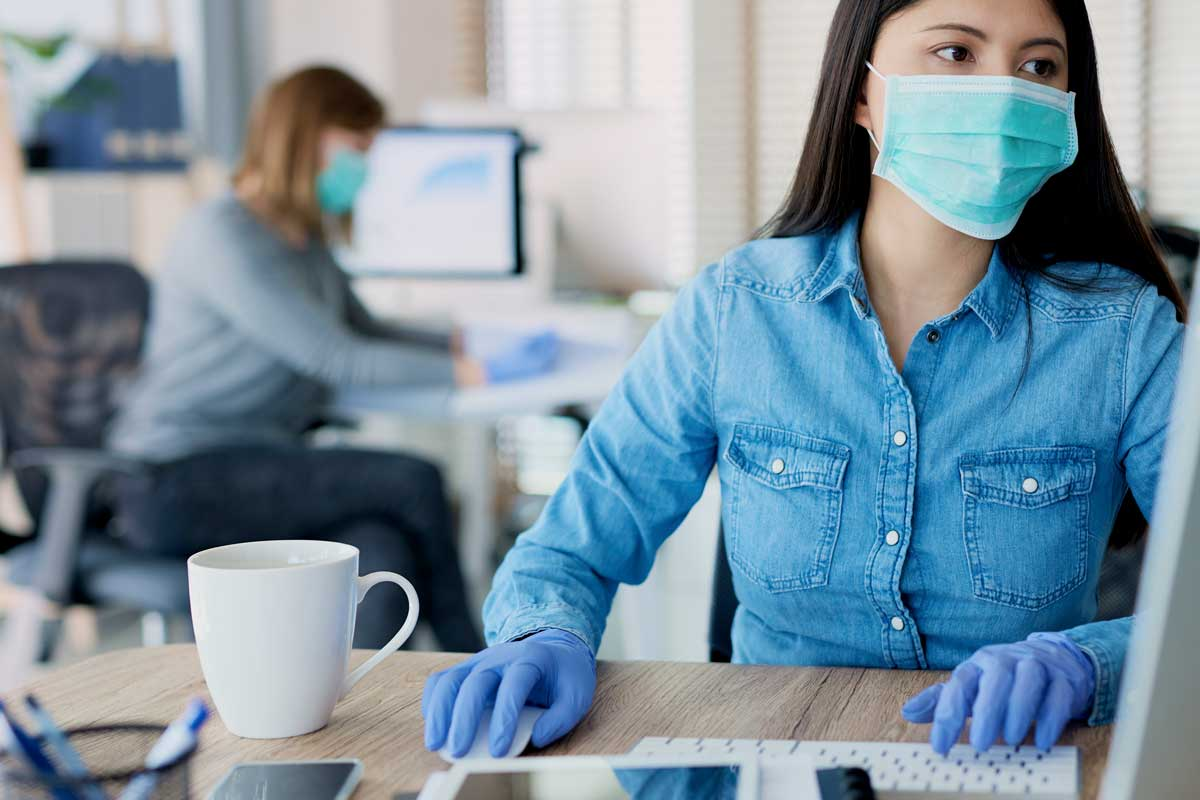
\includegraphics[width=4.5 cm,height=3.5 cm]{office_mask}
    \includegraphics[width=4.5 cm,height=3.5 cm]{no_office_mask}
\end{frame}

\begin{frame}
    \frametitle{Overview}
    MaskifAI is a mask detection web app which can be used by an organization to ensure that their employees wear a mask while entering the workspace.
\end{frame}

\begin{frame}
    \frametitle{Mask Detection}
    \begin{figure}
    \caption{Wearing mask properly}
    \centering
    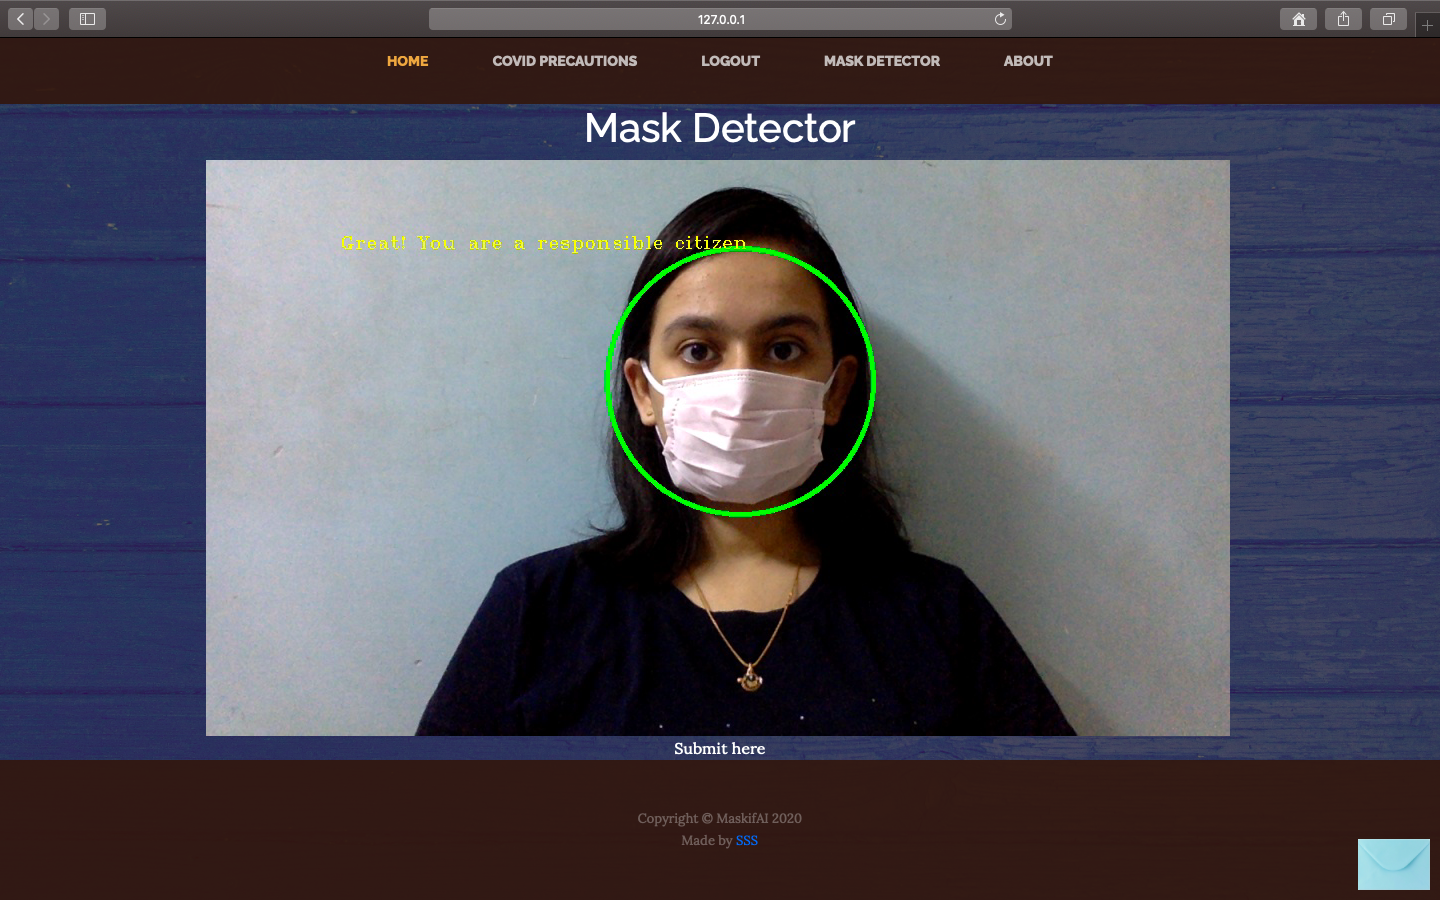
\includegraphics[width=0.75\textwidth]{mask_true}
    \end{figure}
\end{frame}

\begin{frame}
    \frametitle{Mask Detection}
    \begin{figure}
    \caption{Wearing mask improperly}
    \centering
    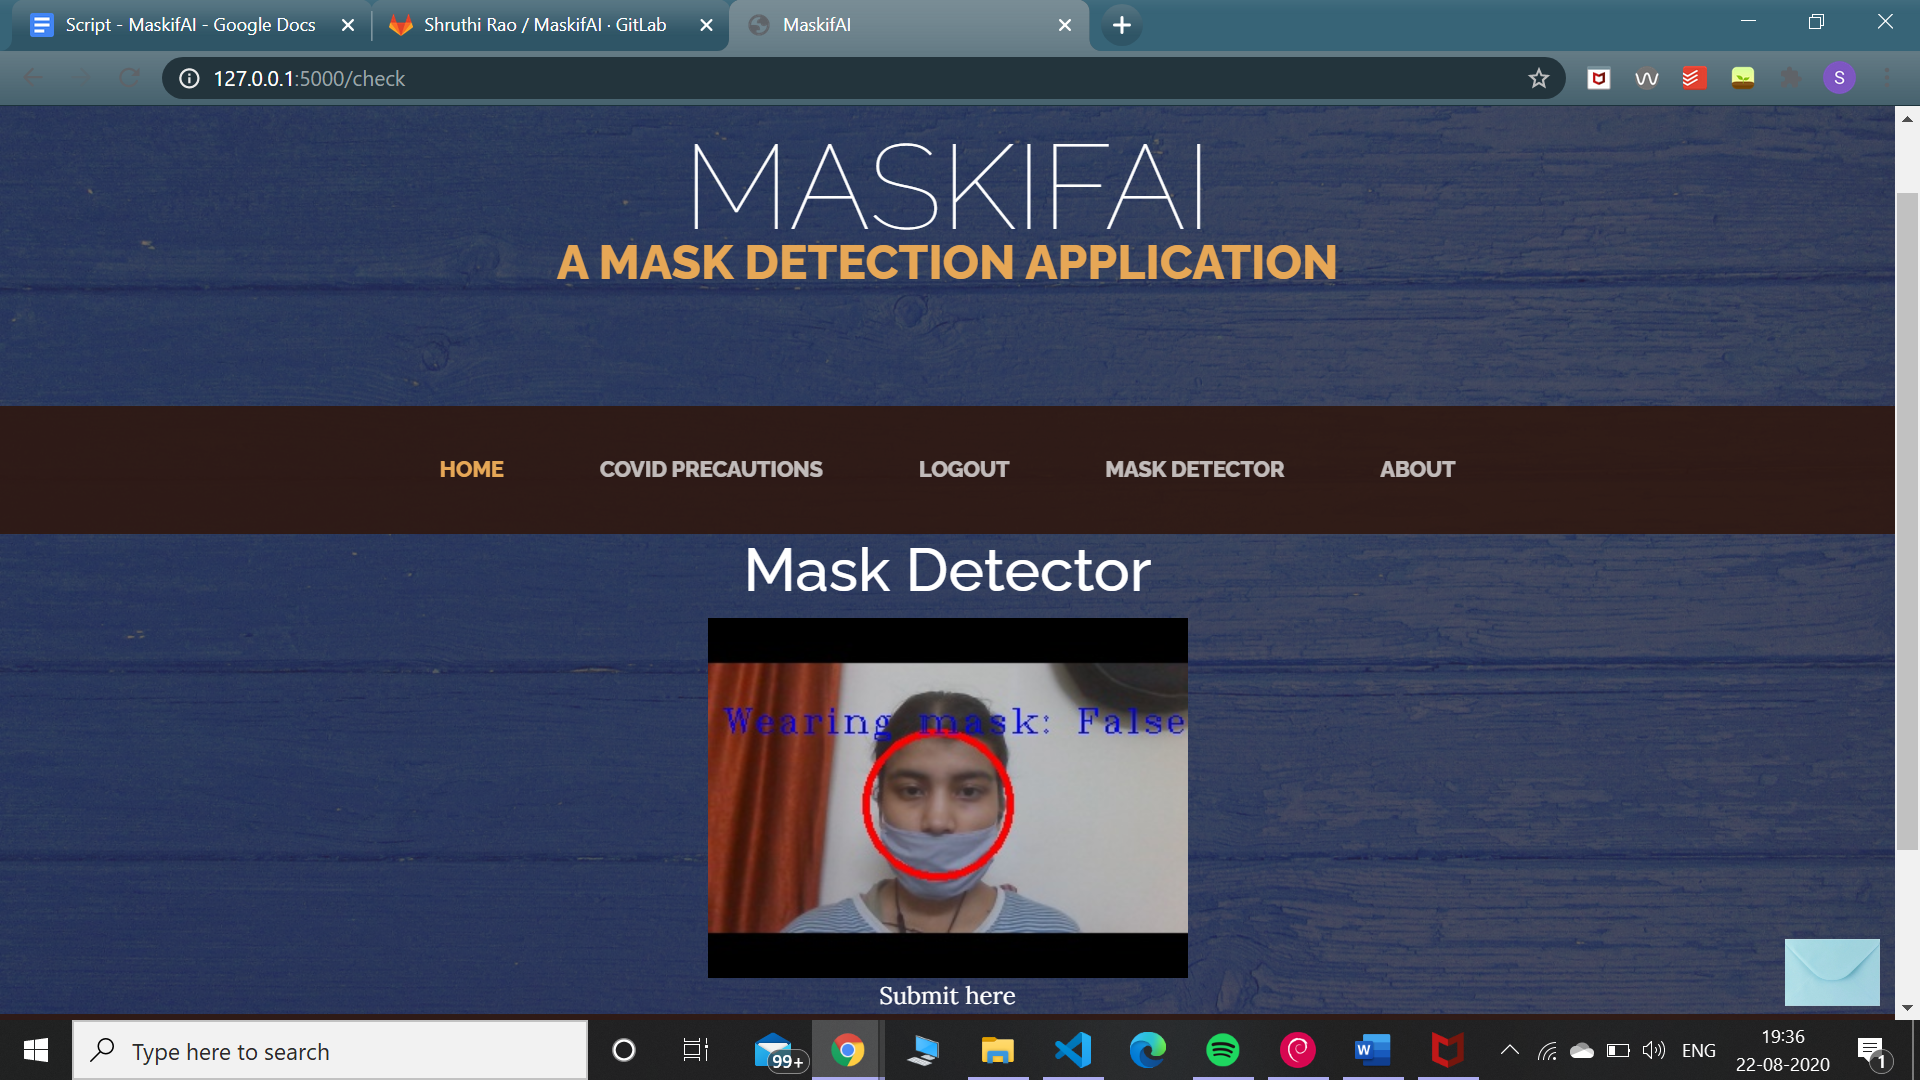
\includegraphics[width=0.8\textwidth]{improper_mask}
    \end{figure}
\end{frame}

\begin{frame}
    \frametitle{Mask Detection}
    \frametitle{Mask Detection}
    \begin{figure}
    \caption{Not Wearing mask}
    \centering
    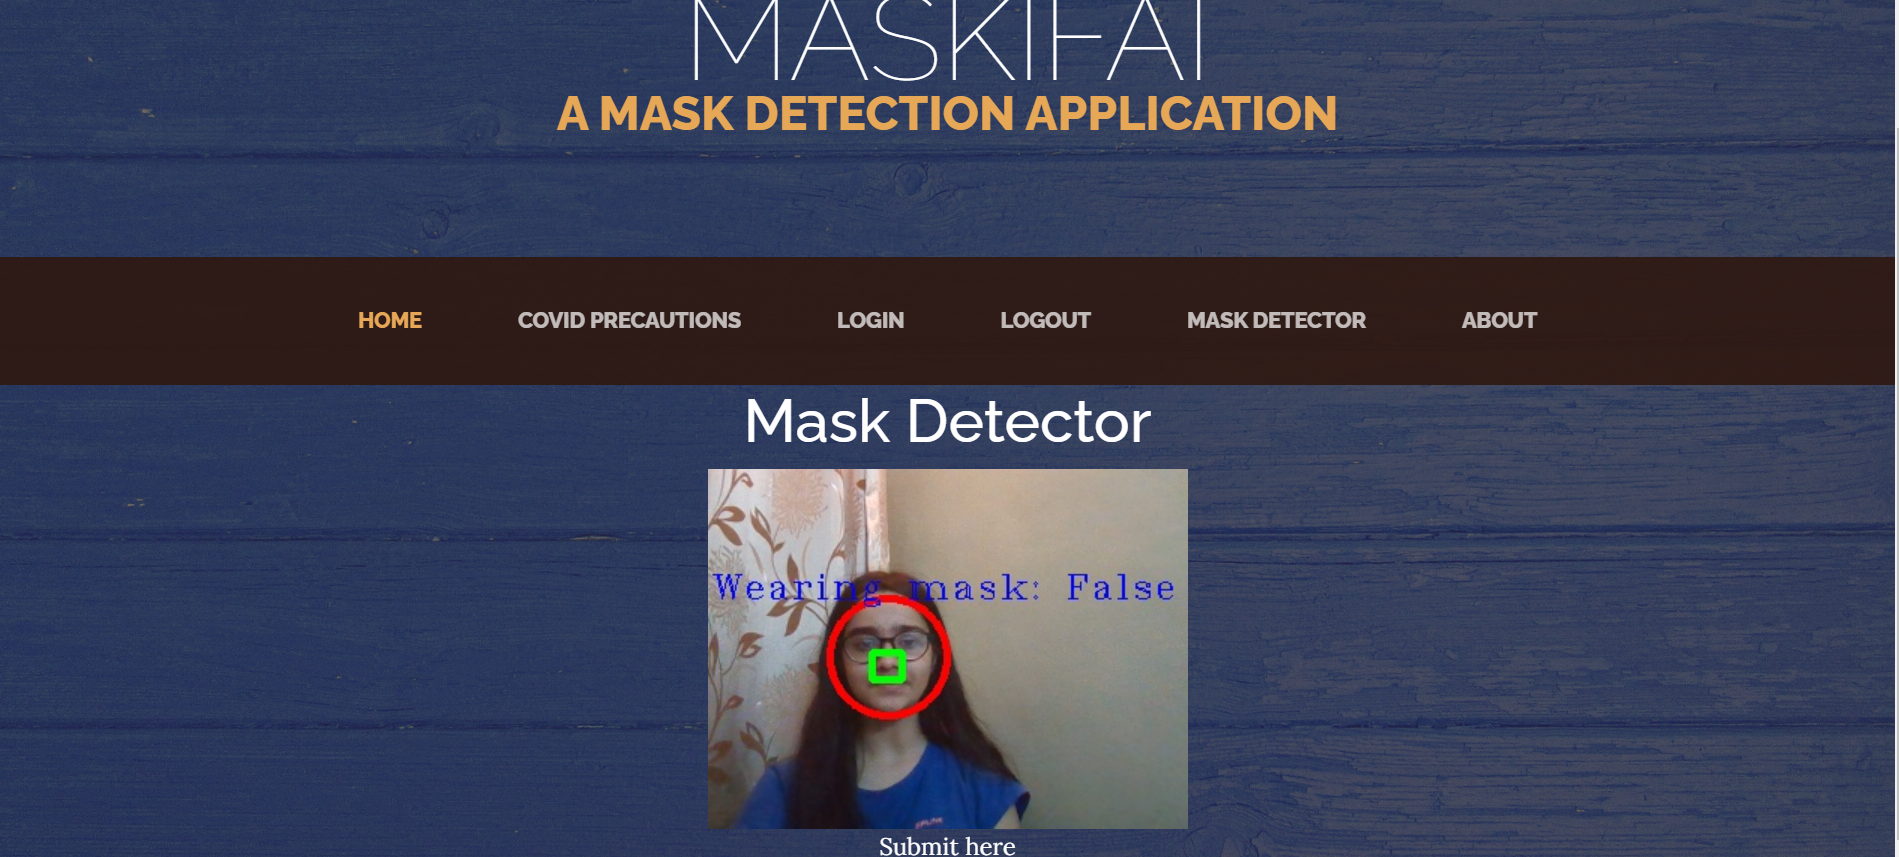
\includegraphics[width=0.8\textwidth]{no_mask}
    \end{figure}
\end{frame}

\begin{frame}
    \frametitle{Tech Stack}
    \begin{enumerate}
        \item Python
        \item OpenCV
        \item Flask
        \item SQLite
        \item HTML/CSS
        \item Bootstrap
    \end{enumerate}
\end{frame} 

\begin{frame}
    \frametitle{Description}
    \begin{enumerate}
        \item App connected to company's authorization system
        \item Employees: Verify if ze is wearing a mask properly
        \item Mask not detected: Admin notified
        \item General hygiene and precautions for Covid-19
    \end{enumerate}
\end{frame}


\begin{frame}
    \frametitle{Target Audience}
    The web application is aimed at helping \textcolor{blue}{organizations} take precautions against Covid-19 by ensuring that all the employees who enter the workspace wear masks.
\end{frame}

% \begin{frame}
%     \frametitle{Statistics}
%     \begin{enumerate}
%         \item 7000 Nose samples
%         \item 3345 sub-classifiers - Nose classifier
%         \item 1047 sub-classifiers - Face classifier
%     \end{enumerate}
% \end{frame}

\begin{frame}
    \frametitle{Challenges}
    \begin{enumerate}
        \item Mask Detection Accuracy
            \begin{itemize}
            \item Eyes and mouth Haar Cascades
            \item Nose Haar Cascade
            \end{itemize}
        \item Using the mask data
        \item Email Notification 
    \end{enumerate}
\end{frame}


\begin{frame}
    \frametitle{Learnings}
    \begin{enumerate}
        \item Pre-trained classifiers: Feature detection
        \item Working with Flask for web development
        \item Front-end
        \item Version control  
        \item Teamwork
    \end{enumerate}
\end{frame}



\begin{frame}
    \frametitle{Future Scope}
    \begin{enumerate}
        % \item Deployment + Web Push notifications
        \item Improve accuracy through Deep Learning
        \item Detect industry-specific protective gear
    \end{enumerate}
\end{frame}

\begin{frame}
    \frametitle{References}
    \begin{enumerate}
        \item \href{https://opencv.org/}{OpenCV documentation} 
        \item \href{https://flask.palletsprojects.com/en/1.1.x/}{Flask documentation} 
        \item \href{http://alereimondo.no-ip.org/OpenCV/uploads/37/CameraReadyPaper63.pdf}{Face and Facial Feature Detection Evaluation  \newline - M. Castrillon-Santana, O. Deniz-Suarez, L. Anton-Canalıs and J. Lorenzo-Navarro}
    \end{enumerate}
\end{frame}

\begin{frame}[c]{ }
    \centering
\huge \textbf{Demo}
\end{frame}
\begin{frame}[c]{ }
    \centering
\huge \textbf{Thank You!}
\end{frame}
\end{document}
